\chapter{實驗結果}\label{result}

\section{水之呼吸}
\begin{itemize}
\item 壹之型 水面斬
\item 貳之型 水車
\item 叄之型 流流舞
\item 肆之型 打擊之潮
\item 伍之型 旱天的慈雨
\item 陸之型 扭轉旋渦
\item 柒之型 雫波紋擊刺·曲
\item 玖之型 水流飛沫·亂
\item 拾之型 生生流轉
\item 組合技——陸之型+叄之型——扭轉旋渦·流流
\item 創新技——貳之型·改——橫水車
\item 拾壹之型 凪
\end{itemize}

\clearpage

\subsection{程式碼範例}

\begin{lstlisting}[language=C]
   /* 範例就來個熟悉的 Hello world */

   int main(int argc, char ** argv) 
   { 
      printf("Hello_world!\n");
      return EXIT_SUCCESS; 
   }
\end{lstlisting}


\begin{figure}

   圖片插入範例 2:\\
   \centering
   
\includegraphics[width=8cm]{../Figures/Result/我就爛}
   \caption{我就爛}\label{fig:我就爛}

   \subfigure[你也爛]{
      
\includegraphics[width=4cm]{../Figures/Result/你也爛}
      \hspace{0.5 in}
   }
   \subfigure[一起爛]{
      
\includegraphics[width=4cm]{../Figures/Result/一起爛}
   }
   \caption{爛起來}\label{fig:爛起來}
\end{figure}

繪圖範例2:
\begin{center}
    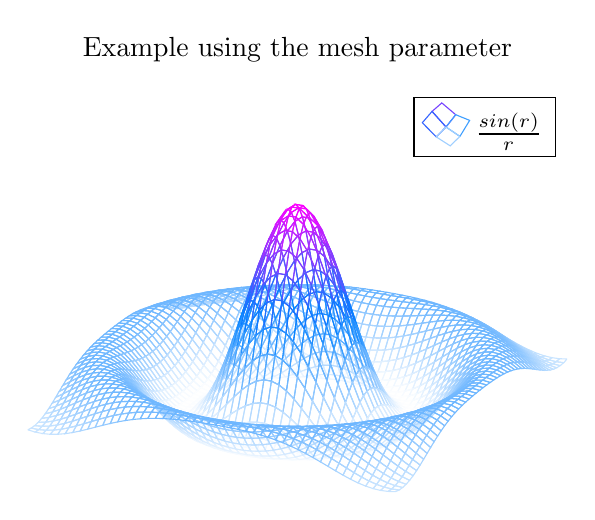
\begin{tikzpicture}
        \begin{axis}[
            title=Example using the mesh parameter, % 圖標題
            hide axis,                              % 隱藏座標
            colormap/cool,                          % 顏色風格
        ]
        \addplot3[
            mesh,                                   % 繪製的三維圖像是網格
            samples=50,                             % 定義域分割數量
            domain=-8:8,                            % 定義域
        ]
        {sin(deg(sqrt(x^2+y^2)))/sqrt(x^2+y^2)};    % 二元顯式函數
        \addlegendentry{$\frac{sin(r)}{r}$}         % 添加圖例
        \end{axis}
        \end{tikzpicture}
\bfseries
\end{center}
